\documentclass{article}
\usepackage[margin=1in]{geometry}
\usepackage{amsmath}
\usepackage{graphicx}
\usepackage{float}
\usepackage{listings}
\usepackage{xcolor}

\lstset{
    language=Matlab,
    basicstyle=\ttfamily\footnotesize,
    keywordstyle=\color{blue},
    breaklines=true
}

\begin{document}

\section*{Problem 1(c)}

To find the scale factor $s$ that minimizes the pointwise error for the nonuniform mesh with $E=20$ elements, a parameter sweep is performed for $s \in [0.5, 0.95]$. For each value of $s$, the mesh is generated, the finite element system is assembled and solved, and the maximum pointwise relative error is computed.

\subsection*{Results}
The parameter sweep reveals a distinct minimum in the error curve. The optimal scale factor is found to be \textbf{0.65}, which yields a minimum maximum pointwise relative error of \textbf{0.0088} ($8.8193 \times 10^{-3}$). This value optimally balances the resolution within the steep boundary layer against the resolution in the remainder of the domain.

\begin{figure}[H]
    \centering
    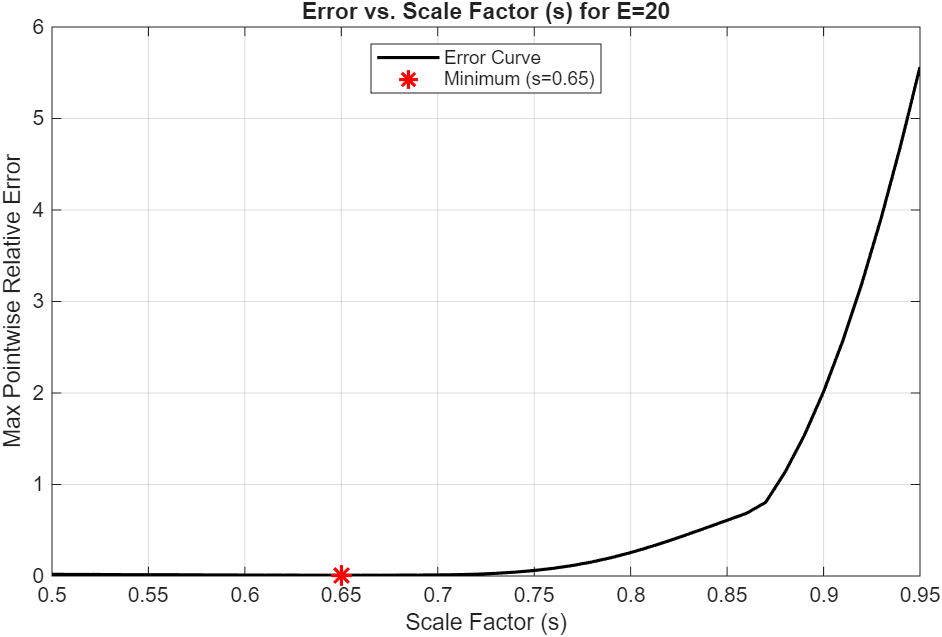
\includegraphics[width=0.7\textwidth]{1_c.png}
    \caption{Error vs. Scale Factor (s) for $E=20$, showing the minimum at $s=0.65$.}
    \label{fig:1c}
\end{figure}

\subsection*{MATLAB Implementation}
\begin{lstlisting}
L = 1.0; c = 1.0; nu = 1e-3; f = 1.0;
E = 20; N = E + 1;

s_vals = 0.5:0.01:0.95;
errors = zeros(length(s_vals), 1);

for k = 1:length(s_vals)
    s = s_vals(k);
    
    L1 = L * (1 - s) / (1 - s^E);
    Le = L1 * s.^(0:E-1);
    x = [0, cumsum(Le)]';
    
    K = sparse(N, N);
    F = zeros(N, 1);
    
    for e = 1:E
        h_e = Le(e);
        A_e = (1.0 / h_e) * [1.0, -1.0; -1.0, 1.0];
        C_e = 0.5 * [-1.0, 1.0; -1.0, 1.0];
        idx = [e, e+1];
        K(idx, idx) = K(idx, idx) + nu * A_e + c * C_e;
        F(idx) = F(idx) + (f * h_e / 2.0) * [1.0; 1.0];
    end
    
    K(1, :) = 0.0; K(1, 1) = 1.0; F(1) = 0.0;
    K(end, :) = 0.0; K(end, end) = 1.0; F(end) = 0.0;
    
    u_h = K \ F;
    
    u_ex = x - exp((c / nu) * (x - L));
    u_ex(1) = 0.0; u_ex(end) = 0.0;
    
    interior_idx = 2:(N-1);
    rel_error = abs(u_ex(interior_idx) - u_h(interior_idx)) ./ abs(u_ex(interior_idx));
    errors(k) = max(rel_error);
end

[min_err, min_idx] = min(errors);
opt_s = s_vals(min_idx);

fprintf('Optimal s value: %.2f\n', opt_s);
fprintf('Minimum maximum pointwise relative error: %.4e\n', min_err);
\end{lstlisting}

\end{document}